\documentclass[landscape,a0,final]{a0poster}
\usepackage[dvipsnames,svgnames]{xcolor}
\usepackage{minted} %code highlighting, not working yet
\usepackage{tikzposter} % here most of the things are defined
% change parameters only after this line You can also start a new column with an arbitrary 
% x-coordinate by specifying explicitly the coordinate of the new block node as follows:
\usepackage[czech]{babel}
\usepackage[utf8]{inputenc}
\usepackage{wrapfig}
\usepackage{url}

%Used for better control on code display

\usepackage[margin=\margin cm, paperwidth=197cm, paperheight=100cm]{geometry}

% \setbackgrounddarkcolor{ForestGreen!70!black}
% \setbackgroundlightcolor{YellowGreen!90!}

% \setfirstcolor{YellowGreen!80!}
% \setsecondcolor{gray!80!}
% \setthirdcolor{red!80!black}

\title{From Water Dynamics to Rainfed Landscapes with GRASS GIS\bigskip}
\author{Yann Chemin$^1$, Martin van Brakel$^2$, Robyn Johnston$^1$, Jayne Curnow$^1$\\
\bigskip
\\ $^1$International Water Management Institute, $^2$CRP on Water, Land and Ecosystems (WLE)}

\usetemplate{1}
\setinstituteshift{1}

\setblocktitleheight{2}
\setblockspacing{1}

\begin{document}
\ClearShipoutPicture
\AddToShipoutPicture{\BackgroundPicture}
\noindent
\tikzstyle{every picture}+=[remember picture]
\begin{tikzpicture}
\initializesizeandshifts
\titleblock{120}{1}
% \setblocktitleheight{1}
\addlogo[north west]{(2,-1)}{9cm}{./svg_images/Grass_GIS.pdf}
\addlogo[north west]{(13,-3)}{19cm}{./svg_images/OSGeo_logo.pdf}
\addlogo[north east]{(-2,-4.5)}{30cm}{./images/CR10583_1wle-iwmi_logo}

%%%%%%%%%%%%%%%%%%%%%%%%%%%%%%%%%%%%%%%%%%%%%%%%%%%%%%%%%%%%%%%%%%%%%%%%%%%%%%%%
\blocknode{Abstract}{
\small \noindent Variability in water availability is a key determinant of risk and constraint to productivity in rainfed agricultural systems. Understanding the dynamics of water availability across both spatial and temporal scales is essential to managing water and optimize production. This research proposes to look at both the physical measurement of water availability and water user perceptions of landscapes and water availability.\newline\linebreak
\noindent Evapotranspiration makes up about three quarters of the transiting water in a landscape, it is composed of evaporation (water bodies, soil) and transpiration, the vegetation biomass growing quantity. This work will develop a methodology for defining landscapes based on water dynamics to be used at the interface of WLE research. The GRASS GIS [1] Imagery (i.*), Landscape (r.li.*) and Temporal (t.*) toolkits form the basis of the methodological development, from evapotranspiration modeling and landscape analysis to spatio-temporal analysis.\newline\linebreak
The methodology will be complemented by time series analysis spanning 14 years up to near real-time (2000-2014) of MODIS vegetation index data, capable of distinguishing seasonal and long term land use and land cover trends in these landscapes. This analysis will be developed into a routine that can be executed in open source GIS (GDAL [2] tools and GRASS GIS [1]), providing a robust and readily available application for monitoring medium to large scale land use and land cover change over any desired area.
}

%%%%%%%%%%%%%%%%%%%%%%%%%%%%%%%%%%%%%%%%%%%%%%%%%%%%%%%%%%%%%%%%%%%%%%%%%%%%%%%%
\blocknode{Transpiration and the search for rainfed landscapes}{
\smallskip
\begin{center}
	\begin{tabular}{c p{0.5\textwidth}}
	 \raisebox{-0.9\totalheight}{\includegraphics[width=0.45\textwidth]{./images/Yann_flowchart}}
	&
	The transpiration data is created from energy balance modelling [3] modules (i.eb.*, i.evapo.*) within GRASS GIS version 7, by partitioning the net radiation (r.sun) into soil heat flux (i.eb.soilheatflux), sensible heat flux (i.eb.h\_*) and the residual being the energy needed to evaporate water (i.eb.evapfr, i.eb.eta). This information is then fractionated into biotic (transpiration) and abiotic (evaporation) parts using vegetation fraction.\newline\linebreak
The accumulated transpiration (t.rast.aggregate) is subjected to Landscape analysis (r.li.*) for search of patchiness and diversity indices [4]. Further analysis of transpiration is also done with the object oriented classifier (i.segment) for spatiotemporal objects within the transpiration original dataset, the accumulated one and the Landscape indices, respectively.\newline
 	\end{tabular}\newline
\end{center}
\begin{center}
	\begin{tabular}{cc}
 	\includegraphics[width=0.45\textwidth]{./images/RGB321_PCA_Ta_2000}
 	& 
 	\includegraphics[width=0.45\textwidth]{./images/SEG_PCA_Ta_2000}
	\end{tabular}
\end{center}
Using the 50 first PCA components of the Transpiration data for year 2000, the object types that can be extracted by object-based classification were analysed. It turns out that the recession cropping around Tonle Sap and the rainfed cropping systems of Eastern Thailand are clearly extracted. However, the recession cropping in Tonle Sap only has one main class, which is different when using 2000-2014 EVI PCA classification (central part of the poster). It is thought that both the 500x500m resolution and the yearly changes in flooding height in Tonle Sap are driving the separation of the recession cropping area, thus not seen here with one year (2000) and 1x1km pixel size.\newline
}


%%%%%%%%%%%%%%%%%%%%%%%%%%%%%%%%%%%%%%%%%%%%%%%%%%%%%%%%%%%%%%%%%%%%%%%%%%%%%%%%
\getcurrentrow{box}
\coordinate (funkcionalita) at (box.south west);
\coordinate (funkcionalitaeast) at (box.east);
\coordinate (screenshot) at (box.north west);

\blocknodew[($(funkcionalita)+(20,-1)$)]{35}{References}{
\scriptsize
\begin{center}
\begin{tabular}{rp{0.9\textwidth}}
[1] & Neteler \& Bowman \&  Landa \& Metz, 2012. Environment \& Modeling Software, 31:124-130\\{}
[2] & GDAL, 2014. {\url {http://gdal.osgeo.org}}\\{}
[3] & Chemin, 2012. Chapter 19, DOI: 10.5772/23571 ({\url {http://bit.ly/16qJOep}})\\{}
[4] & McGarigal \& Marks, 1995. FRAGSTATS. USDA For. Serv. Gen. Tech. Rep. PNW-351.\\{}
[5] & Momsen \& Metz, 2012. GSoC project: Segmentation algorithm.\\{}
[6] & Eastman \& Fulk, 1993. Photogramm. Eng. Remote Sens. 59(8), 1307-1312.
\end{tabular}
\end{center}
\smallskip
\hrulefill
\vspace{-5pt}

\begin{center}
\begin{tabular}{cp{0.9\textwidth}}
\begin{minipage}{0.15\textwidth}
\includegraphics[width=0.7in]{./images/iwmi_qr.pdf}
\end{minipage}

\begin{minipage}{0.3\textwidth}
\small {\url{www.iwmi.org}}
\end{minipage}

\begin{minipage}{0.15\textwidth}
\includegraphics[width=0.7in]{./images/grass_qr.pdf}
\end{minipage}

\begin{minipage}{0.3\textwidth}
\small {\url{grass.osgeo.org}}
\end{minipage}
\end{tabular}
\end{center}

\hrulefill
\vspace{14pt}
\begin{center}
\newcommand{\logowidth}{5em}
\newcommand{\logospace}{\hspace{0.1em}}
\noindent
\includegraphics[width=\logowidth]{./svg_images/public_domain_logo.pdf}
\raisebox{0.7\height}{\logospace 2013 GRASS Development Team}
\end{center}
}

\startsecondcolumn


%%%%%%%%%%%%%%%%%%%%%%%%%%%%%%%%%%%%%%%%%%%%%%%%%%%%%%%%%%%%%%%%%%%%%%%%%%%%%%%%
\blocknode{Temporal PCA-based classification}{
\smallskip
\begin{center}
	\begin{tabular}{c p{0.5\textwidth}}
	\raisebox{-0.9\totalheight}{\includegraphics[width=0.45\textwidth]{./images/Martin_flowchart}}
	&
	Long sequence time series PCA provides a comprehensive indicator of change events in time series of spatial environmental data (Eastman \& Fulk 1993)1. Principal Components Analysis undertakes linear transformation of a set of image bands to create a new set of images that are uncorrelated. This set of principal component images can be considered equivalent to bands of a multi-spectral image. Each image represents a different portion of spectral variability in the original image data set. The clusters yielded by subjecting the PCA component images to iterative self-organising cluster routine each express a particular signature, corresponding to a unique combination of characteristics in terms of the environmental variable under study.\newline
 	\end{tabular}\newline
\end{center}
The methodology involves the following steps: 1) a time series of EVI composites is subjected to PCA; 2) the Principal Component images explaining most (ca. 95\%) of spatio-temporal variation in the time series, are used as input layers or ‘bands’ in the iterative self-organising cluster routine; 3) for each spatial cluster in the image output a Boolean mask is created and 4) overlaid (multiplied) with the original time series, which results in 5) a VI time series for each cluster in the output. Analysis of the temporal signature for each cluster reveals seasonal or long-term trends in VI that occur within the system.
%A summary of the code needed to reach this point of analysis is here.\newline
%{\footnotesize \fontfamily{pcr}\selectfont i.group \textcolor{blue}{group}=pca\_group \textcolor{blue}{input}=\$(g.mlist \textcolor{blue}{type}=rast \textcolor{blue}{pattern}=*h28v07*EVI)\newline
%i.pca \textcolor{blue}{input}=pca\_group \textcolor{blue}{output\_prefix}=pca\_ \textcolor{blue}{percent}=99 --o\newline}

%Minted version Not working (+ compile needs -shell-escape)
%\begin{minted}[frame=single,linenos,mathescape,fontsize=\small]{sh}
%	i.group group=pca_group input=$(g.mlist type=rast pattern=*h28v07*EVI)
%	i.pca input=pca_group output_prefix=pca_ percent=99 --o
%\end{minted}
}

%%%%%%%%%%%%%%%%%%%%%%%%%%%%%%%%%%%%%%%%%%%%%%%%%%%%%%%%%%%%%%%%%%%%%%%%%%%%%%%%
\blocknode{Temporal PCA-based classification}{
\begin{center}
	\begin{tabular}{cc}
 	\raisebox{-0.5\totalheight}{\includegraphics[width=0.45\textwidth]{./images/MSUBAS_MD}}
 	& 
 	\begin{tabular}{c}
 	\includegraphics[width=0.45\textwidth]{./images/cl2_DoY}\\
 	\includegraphics[width=0.45\textwidth]{./images/cl12_DoY}
	\end{tabular}
	\end{tabular}
\end{center}
This application employs a time series of MODIS EVI 16-day composites at 500 m resolution (MOD13A1) running over 14 years (2000 to near real-time). The h28v07 tile covers large part of the Mekong River Basin in Southeast Asia. We analyse a subset covering the Vietnamese Mekong Delta (VMD) and the Tonle Sap in Cambodia (TSC). \newline
The results discern large areas in VMD dominated by irrigated triple crop rice agro-ecosystems, followed by seasonal flooding near the end of each year, as well as long-term change from double cropping to triple cropping in adjacent areas from 2008 onward.\newline
}

\startthirdcolumn

%%%%%%%%%%%%%%%%%%%%%%%%%%%%%%%%%%%%%%%%%%%%%%%%%%%%%%%%%%%%%%%%%%%%%%%%%%%%%%%%
\blocknode{Temporal patterns of recession cropping \& natural vegetation}{

\begin{center}
	\begin{tabular}{cc}
	\raisebox{-0.5\totalheight}{\includegraphics[width=0.45\textwidth]{./images/MSUBAS_TS}}
	&
	\begin{tabular}{p{0.5\textwidth}}
 	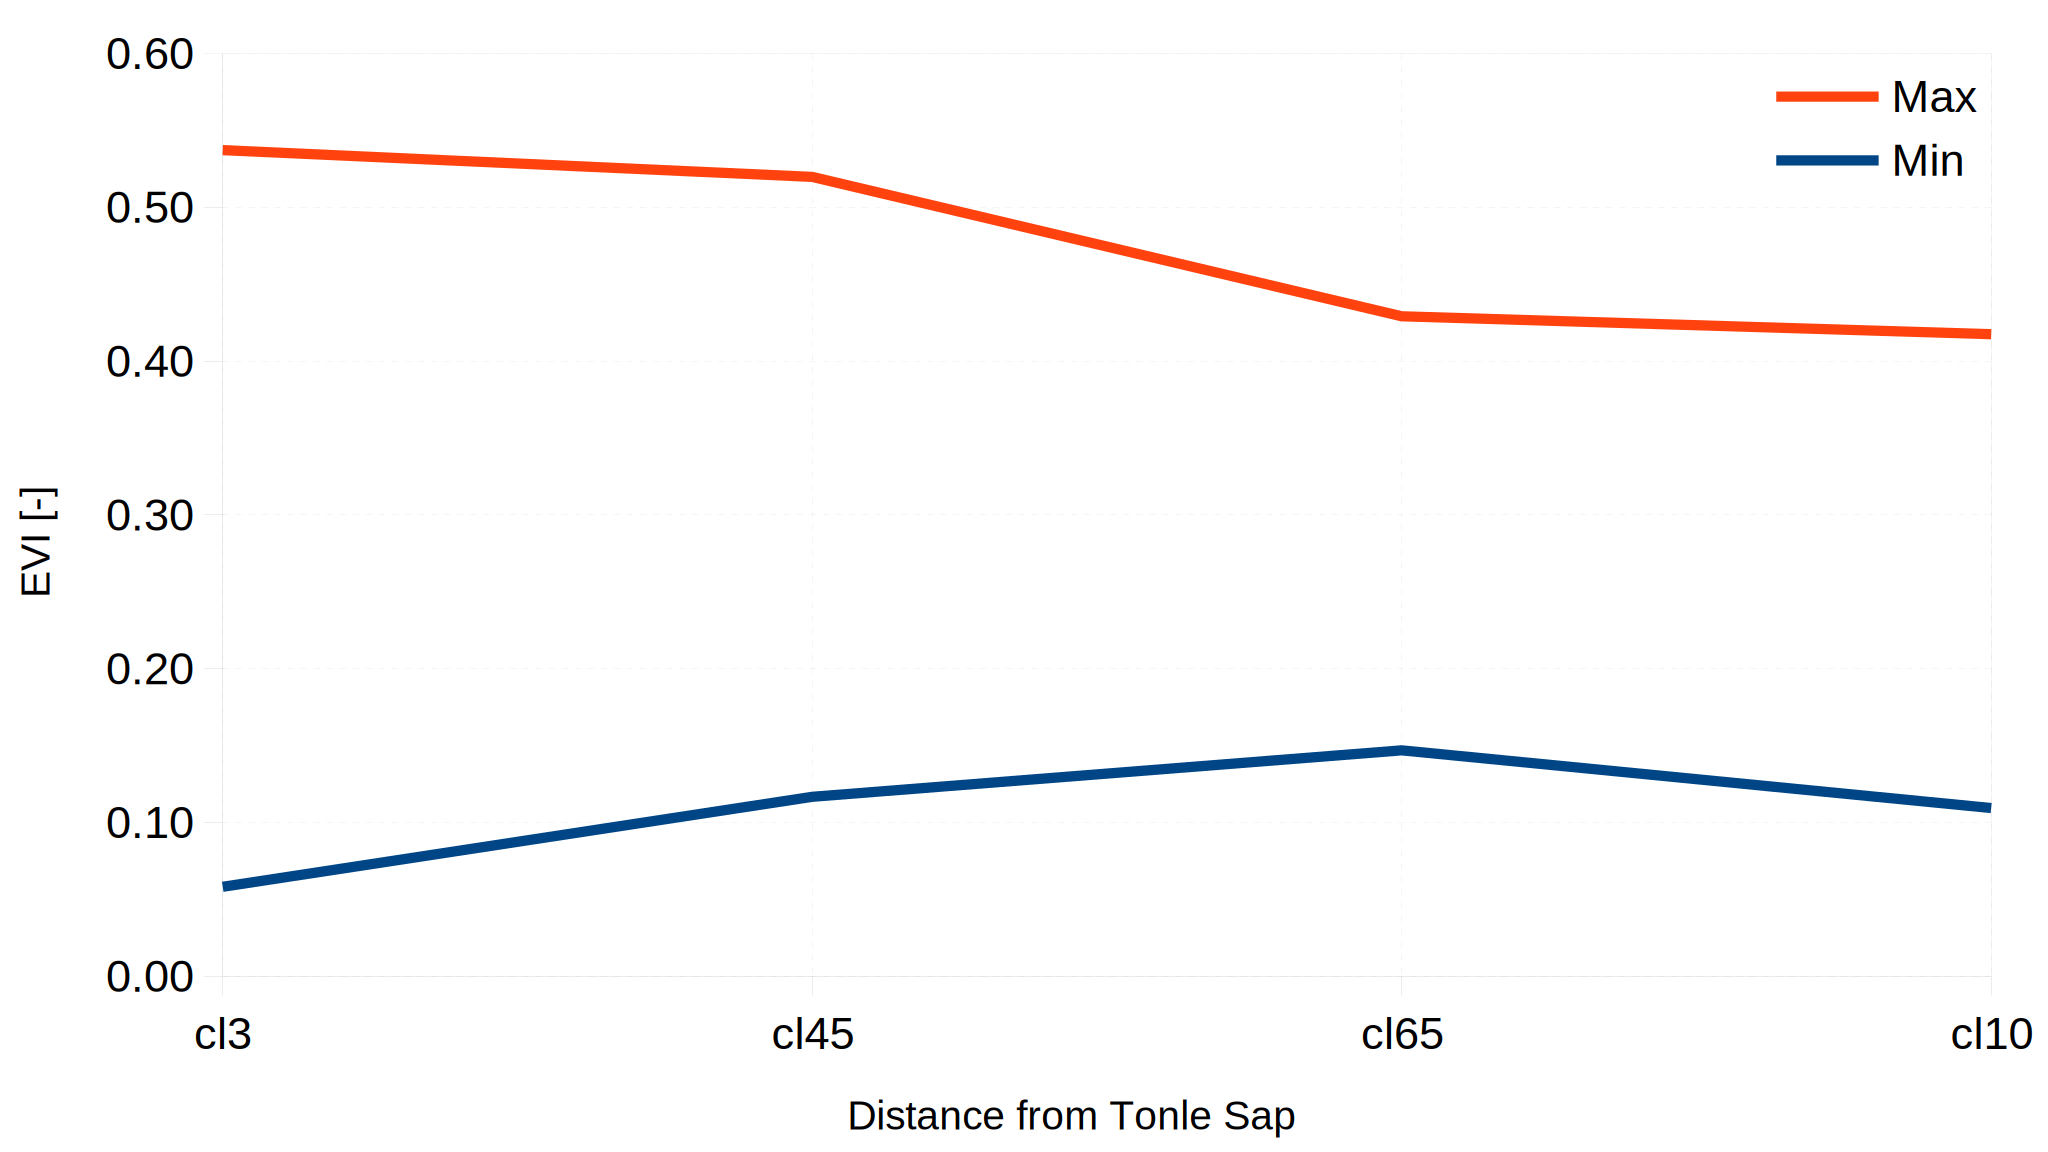
\includegraphics[width=0.45\textwidth]{./svg_images/EVI_distance_from_tonle_sap}\\
	The results for TSC show that the range between $EVI_{min}$ and $EVI_{max}$ in floodplains surrounding the Tonle Sap Lake decreases spatially with distance from dry season margins of the lake. This pattern is indicative of flood recession cropping systems and seasonally flooded natural vegetation around the lake, which expands dramatically in size during the wet season each year, inundating large areas of floodplain, which drain towards the dry season.  We used the blue band of MOD13 to provide an additional indicator of flooding, handling the assumption of seasonal flood occurrence if ‘Blue’ approaches or exceeds ‘EVI’. The results in TSC do not discern any long-term trends in land cover and land use.\newline
	\end{tabular}
 	\end{tabular}\newline
\end{center}

}

%%%%%%%%%%%%%%%%%%%%%%%%%%%%%%%%%%%%%%%%%%%%%%%%%%%%%%%%%%%%%%%%%%%%%%%%%%%%%%%%
\blocknode{Recession cropping \& natural vegetation}{
\begin{center}
	\begin{tabular}{cc}
 	\begin{tabular}{c}
 	\includegraphics[width=0.5\textwidth]{./images/cl3_avg}\\
 	\includegraphics[width=0.5\textwidth]{./images/cl65_avg}
	\end{tabular}
 	& 
 	\begin{tabular}{c}
 	\includegraphics[width=0.5\textwidth]{./images/cl45_avg}\\
 	\includegraphics[width=0.5\textwidth]{./images/cl10_avg}
	\end{tabular}
	\end{tabular}\newline
\end{center}

}



\startfourthcolumn

%%%%%%%%%%%%%%%%%%%%%%%%%%%%%%%%%%%%%%%%%%%%%%%%%%%%%%%%%%%%%%%%%%%%%%%%%%%%%%%%
\blocknode{Euclidian Distance plotting}{
\smallskip
The Euclidian distance plot depicts graphically the resemblance between spatio-temporal signatures of the systems under study. Similar landscape groups can be distinguished at Euclidean distance of 2.1 or less.  Euclidean distance of 1.1 or less assumes that dissimilarity between systems is not statistically significant at that level. \newline
\begin{center}
	\includegraphics[width=0.75\textwidth]{./images/msubas65}
\end{center}

}
%%%%%%%%%%%%%%%%%%%%%%%%%%%%%%%%%%%%%%%%%%%%%%%%%%%%%%%%%%%%%%%%%%%%%%%%%%%%%%%%
\blocknode{Biotic Zoning}{
\smallskip
Object based classification (\textit{i.segment}) of the sum transpiration for each year has been done and merged, resulting areas were clumped (\textit{r.clump}) and averaged statistics of yearly transpiration extracted (\textit{r.stats.zonal}).\newline
Rainfed cropping in Isarn (Part 1) is clearly identified as low transpiration signal (red colour), Recession cropping areas around Tonle Sap (Part 2 \& 3) are high signals (Blue and green) with both noise and a negative impact on transpiration in Part 2 around mid-year (Green signal drop). A southern area (Part 4) of most probably rainfed benefiting from flood to some extent to propose some kind of recession cropping with a mid-year transpiration raise signal (Violet).\newline
\begin{center}
	\begin{tabular}{cc}
 	\begin{tabular}{p{0.5\textwidth}}
 	\includegraphics[width=0.45\textwidth]{./images/seg_ta_years_clump_reclass_ta_avg}\\
 	\vspace{5mm}
 	This perspective proposes that irrigated areas along the Mekong may not be transpiring as much as the recession cropping areas around Tonle Sap. Whether the transpiration in recession zones is actually used by crops all the time depends on the opportunity of farming intensification and risk avoidance.\newline 
	\end{tabular}
 	& 
 	\begin{tabular}{c}
 	\includegraphics[width=0.45\textwidth]{./images/Ta_loc}\\
 	\includegraphics[width=0.45\textwidth]{./images/Ta}
	\end{tabular}
	\end{tabular}
\end{center}
}

\end{tikzpicture}

\end{document}
